%-----------------------------------------------------------------------------
%  Copyright (C) 2004-2017 Andrew Mathas, University of Sydney
%
%  Distributed under the terms of the GNU General Public License (GPL)
%                  http://www.gnu.org/licenses/
%
% This file is part of the MathQuiz system.
%
% <Andrew.Mathas@sydney.edu.au>
%-----------------------------------------------------------------------------

\synctex=1

\documentclass[svgnames]{article}
\usepackage[a4paper,margin=30mm]{geometry}
\parindent=4mm
\parskip=1mm
\hfuzz 5pt

\usepackage{mathquiz-doc}
\usepackage{xparse}
\usepackage{pdfpages}

\renewcommand*\contentsname{\relax}

% hyperref links to ctan
\NewDocumentCommand\ctan{ O{#2} m}{\href{https://www.ctan.org/pkg/#1}{\texttt{#2}}}

%%%%%%%%%%%%%%%%%%%%%%%%%%%%%%%%%%%%%%%%%%%%%%%%%%%%%%%%%%%%%%%%%%%%%%%%%%%%%%%%%%%%%%%
%% MathQuiz title box for front page
\usepackage{tikz}
\usetikzlibrary{shadows.blur}
\tikzset{shadowed/.style={blur shadow={shadow blur steps=5},
                          bottom color=Wheat,
                          top color=Peru,
                          draw=Sienna,
                          shade,
                          font=\normalfont\Huge\bfseries\scshape,
                          rounded corners=8pt,
      },
      boxes/.style={draw=Sienna,
                    fill=Cornsilk,
                    font=\sffamily\small,
                    inner sep=5pt,
                    rectangle,
                    rounded corners=8pt,
                    text=Brown,
     }
}

\def\MathQuizTitle{
  \begin{tikzpicture}[remember picture,overlay]
      \node[yshift=-3cm] at (current page.north west)
        {\begin{tikzpicture}[remember picture, overlay]
          \draw[shadowed](30mm,0) rectangle node[white]{MathQuiz} (\paperwidth-30mm,16mm);
          \node[Crimson,font=\normalfont\small\itshape] at (\paperwidth/2,2mm)
          {\small \mathquiz{description}};
          \node[anchor=west,boxes] at (4cm,0cm) {\mathquiz{name}};
          \node[anchor=east,boxes] at (\paperwidth-4cm,0) {Version \mathquiz{version}};
         \end{tikzpicture}
        };
   \end{tikzpicture}
}

\hypersetup{pdftitle={MathQuiz manual}}

%%%%%%%%%%%%%%%%%%%%%%%%%%%%%%%%%%%%%%%%%%%%%%%%%%%%%%%%%%%%%%%%%%%%%%%%%%%%%%%%%%%%%%%
%% headers and footers
\makeatletter
\def\@oddfoot{\tiny\MathQuiz -- \mathquiz{version}\hfill\thepage}
\makeatother

\begin{document}

    \MathQuizTitle

    \begin{quote}
        \MathQuiz makes it possible to write on-line quizzes using
        \LaTeX, providing an easy way for anyone who knows \LaTeX\ to
        create an on-line quiz using \LaTeX\ file.  The
        allows the quiz author to concentrate on the content of quizzes,
        unencumbered by the technicalities of HTML and javascript.

       \ScreenShot{quiz-page}

        \begin{center}
        \begin{minipage}{0.7\textwidth}
          \hspace*{3em}\tableofcontents
        \end{minipage}
        \end{center}

        \bigskip
        \begin{tabular}{@{}ll}
        Authors             & \mathquiz{authors}\\
        Maintainer          &  \mathquiz{name}\\
        System requirements & python3 and \LaTeX, including \TeX 4ht and \textsc{make4ht}\\
        Licence             & \mathquiz{licence}\\
        Date                & \mathquiz{release date}
        \end{tabular}
    \end{quote}


    \newpage

\section{Introduction}
    On-line quizzes provide a good way to reinforce learning, especially
    because they can give ``interactive'' feedback to the students based
    on the answers that they give. Unfortunately, in addition to writing
    the quiz content there are significant technical hurdles that need
    to be overcome when writing an on-line quiz -- and there are
    additional complications if the quiz involves mathematics or
    diagrams. On the other hand, professional mathematicians and
    educators use \LaTeX\ to write their research papers, books and
    teaching materials.  \MathQuiz merges these two paradigms and makes
    it possible to write on-line quizzes in \LaTeX.

    \MathQuiz supports the following three types of questions:
    \begin{itemize}
      \item Multiple choice questions with a unique correct answer
      \item Multiple choice questions zero or more correct answers
      \item Questions with a numerical answer.
    \end{itemize}
    Each time a student answers a questiuon they are told whether they
    are right or wrong and it is possible for the quiz author to give
    targeted feedback to the student based on their answer.

    In principle, the quiz can contain anything that can be typeset
    using \LaTeX.  In practise, the \LaTeX\ is converted to HTML using
    \href{https://www.tug.org/applications/tex4ht/mn.html}{\TeX 4ht} (
    and \href{https://github.com/michal-h21/make4ht}{make4ht}), which are
    packaged with most \TeX\ distributions. The quizzes constructed
    using \MathQuiz can use anything in \LaTeX\ that is understood by
    \TeX 4ht, which is almost everything.

    The easiest way to explain how \MathQuiz works is by example. The
    following \LaTeX\ file defines a quiz with a single multiple choice
    question that has four possible answers, each of which has a
    customised response.  (Responses to answers are optional, but they
    are one of the main pedagogical advantages of on-line quizzes because the
    quiz can explain why the submitted answer was correct or incorrect.)

    \lstinputlisting[style=latexcode]{example}

    Since this is a \LaTeX\ file it can be processed using
    \texttt{pdflatex}, or \texttt{latex}, to produce a readable and
    printable version of the quiz, which can be useful useful when
    proofreading. In this case, the \LaTeX\ version of the quiz looks
    something like this:

    \ScreenShot[0.5]{example-pdf}

    Of course, the real reason for using \MathQuiz is that it is also
    possible to make an on-line version of the quiz by processing the
    quiz using the \texttt{mathquiz} command. If you do this, and then open
    the web page in your favourite browser, you will see a web page
    that looks something like this:

    \ScreenShot{example-html}

    The web page version of the quiz displays one question at a time,
    with the question buttons serving the dual purpose of, first,
    providing a way to navigate between the different questions in the
    quiz and, secondly, displaying whether or not the question has been
    attempted and, if so, whether it answered correctly or incorrectly.
    Targeted feedback can be given to the person taking the quiz based
    on their responses.

    As explained in \autoref{S:documentclass}, it is possible to
    customise some aspects of the web pages constructed by \MathQuiz.
    With some very rudimentary python, it is possible to change the page
    layout of the quizzes or to embed them into you local web pages; see
    \autoref{S:installation}.

\subsection{What MathQuiz does and does not do}

    The quizzes made using \MathQuiz are intended to be used as a
    revision resource rather than as an assessment tool. In particular,
    \MathQuiz does not provide a mechanism for recording the marks
    obtained in quizzes. Technically, it would not be very hard to record marks
    but it would be more difficult to ensure that the quiz content
    content and solutions are secure. Currently the answers to the quiz
    are not part of the HTML source code for the quiz, however, there
    are ways to access the answers if you know when you are doing.

    Each question in a quiz, and each quiz itself, can be attempted as
    many times as the student wants. \MathQuiz does not provide any way
    of limiting the number of times that the questions can be attempted.

    The questions in a \MathQuiz quiz are static. In particular, they do
    not accept variables and exactly the same questions will appear in
    exactly the same order each time the quiz is taken. It would not be
    hard to make the questions appear in a random order. Randomising the
    order of the multiple choice answers would be more be difficult with
    the current implementation.

    \MathQuiz is able to ask ``computational'' questions that accept a
    numerical answer, however, symbolic answers are not supported.
    For example, if the answer to a question is $0$ then $\sin(0)$ will
    not be accented as a correct answer and the only way to ask for the
    indefinite integral of a function is as a multiple choice question.

    The quizzes are not timed.

    Some of these issues may be addressed in future releases.

\subsection{Credits}
    \MathQuiz{} was written and developed in the
    \href{http://www.maths.usyd.edu.au/}{School of Mathematics and
    Statistics} at the \href{http://www.usyd.edu.au/}{University of
    Sydney}.  The system is built on \LaTeX{} with the conversion from
    \LaTeX{} to HTML being done by Eitan Gurari's
    \href{http://www.cis.ohio-state.edu/~gurari/TeX4ht/mn.html}{TeX4ht}
    (and, more recently, Michal Hoftich's
    \href{https://github.com/michal-h21/make4ht}{make4ht}.

    To write quizzes using \MathQuiz it is only necessary to know
    \LaTeX, however, the underlying \MathQuiz system actually has three components:
    \begin{itemize}
      \item A \LaTeX{} document class file, \texttt{mathquiz.cls}, and
      a \TeX 4ht configuration file, \texttt{mathquiz.cfg}, that enable the
      quiz files to be processed by \LaTeX{} and \TeX 4ht, respectively.
      \item A python program, \texttt{mathquiz}, that translates the
      \LaTeX{} into xml, using \TeX 4ht, and then into HTML.
      \item Some javascript and css that controls and styles the quiz web page.
    \end{itemize}

   The \LaTeX{} component of \MathQuiz{} was written by Andrew Mathas
   and the python, css and javascript code was written by Andrew Mathas
   (and Don Taylor), based on an initial protype of Don Taylor's from
   2001.  Since 2004 the program has been maintained and developed by
   Andrew Mathas. Although the program has changed substantially since
   2004 some of Don's code and, in particular, his idea of using
   \TeX 4ht are still very much in use.

   Thanks are due to Bob Howlett for general help with CSS and, for
   Version~5, to  Michal Hoftich for technical advice.

\section{The MathQuiz document class}\label{S:documentclass}

\subsection{MathQuiz environments and commands}
\begin{description}
  \item[$\backslash$BreadCrumb]
     Sets last item in the web page breadcrumb, which refers to the
     current quiz. By default, the breadcrumb is as set to be the
     part of the quiz title, as set by \verb!\title!,
     before the first colon. For example, the title

     \hspace*{20mm}\verb!\title{Quiz 1: Some interesting questions about frogs}!

     sets the breadcrumb to ``Quiz 1''.

  \item[$\backslash$Department]
    The name of the department that runs this unit (for example,
    Mathematics). This appears below the question buttons on the quiz web
    page.

    The department can be set globally using \texttt{mathquiz --edit-settings}.

    Default: \texttt{School of Mathematics and Statistics}

  \item[$\backslash$DepartmentURL]
    The URL for the department that runs this unit. This appears below
    the question buttons on the quiz web page.

    The department URL can be set globally using \texttt{mathquiz --edit-settings}.

    Default: \texttt{http://www.maths.usyd.edu.au}

  \item[$\backslash$QuizzesURL]
    The URL for the suite of quizzes attached to this unit of study. This
    is used in the breadcrumb at the top of the quiz web page.

    Default: \texttt{Unit code???}

  \item[$\backslash$UnitCode]
    The unit of study code for the course that the quiz is attached
    to. This is used in the breadcrumb at the top of the quiz web page.

    Default: \texttt{Unit code???}

  \item[$\backslash$UnitName]
    The name of the unit of study for the course that the quiz is attached
    to. This is used in the breadcrumb at the top of the quiz web page.

    Default: \texttt{Unit name???}

  \item[$\backslash$UnitURL]
    The URL for the unit of study code for the course that the quiz is attached
    to. This is used in the breadcrumb at the top of the quiz web page.

    Default: \texttt{Unit URL???}

  \item[$\backslash$University]
    The university, or institution, that appears below the question
    buttons on the quiz web page.

    The university can be set globally using \texttt{mathquiz --edit-settings}.

    Default: \texttt{University of Sydney}
  \item[$\backslash$UniversityURL]
    The URL for the university, or institution, that appears below the
    question buttons on the quiz web page.

    The university URL can be set globally using \texttt{mathquiz --edit-settings}.

    Default: \texttt{https://www.sydney.edu.au}
\end{description}

\subsection{Quiz index files}

\subsection{MathQuiz class options}

\begin{description}
  \item[pst2pdf] If this class option is given then \MathQuiz\ uses
  \ctan{pst2pdf} to convert all postscript objects in the quiz to
  images. This sometimes fixes issues with diagrams drawn using
  \ctan{pstricks}. This class option is equivalent to the command-line option
  \texttt{--pst2pdf}.

  \item[tikz] This both loads the \ctan[pgf]{tikz} package (so you do
  not need to have \Verb|\usepackage{tikz}| in your \LaTeX\ file). As a
  bonus, the \textsf{tikz} class option also fixes a bug in PGF that
  stops it from working with \TeX 4ht (thanks are due to Michal
  Hoftich!).\footnote{This bug, together with a one-line solution, has
  been reported to the PGF developers but for reasons unknown they have
  not fixed the problem. See
    \href{https://tex.stackexchange.com/questions/386757/work around for bug
    in pgf when used with htlatex}{Work around for bug in pgf when used with htlatex}
  for more details.}
\end{description}

All other class options are passed to the \texttt{article} class, which is
the base class used by \texttt{mathquiz}.

\section{The MathQuiz program}
\subsection{Command line options}

    The following options can either be used inside \Verb|\MathQuiz| to
    control the formatting \textit{locally} for just the unit being


    \begin{description}
       \item[ -h, --help]            list the command-line options and exit
       \item[-p, --pst2pdf]
          Use pst2pdf to fix issues with images generated by pstricks
       \item[-s,--shell-escape]
          Shell escape for htlatex/make4ht
       \item[--initialise]
          Initialise files and setings for mathquiz
       \item[--settings]
          List system settings for mathquiz
       \item[--edit-settings]
          Edit mathquiz settings
       \item[--build MATHQUIZ\_MK4]
          Build file for make4ht. This can be used to add local
          customisations for make4ht.

       \item[-q, --quiet]
          Suppress tex4ht messages (also -qq etc)
       \item[-l LOCAL\_PAGE, --local LOCAL\_PAGE]
          Local python code for generating the quiz web page
    \end{description}

\subsection{System installation and configuration}\label{S:installation}

    To use the system you will need to have all of the following programs installed:
    \begin{itemize}
         \item \LaTeX, \TeX 4ht and \textsc{make4ht}
         All of these are available through standard \TeX\ installations
         such as \TeX live
         \item Python3
         \item \MathQuiz
    \end{itemize}

    \MathQuiz will soon be submitted to ctan, in which case it will soon
    be incorporated into \TeX live.

\subsection{Local customisation}

  The "style" of the online quizzes is controlled by the file
  \verb!mathquiz_local.py!. If you want to change this format of the quiz
  pages then the easiest way to do this is to make a copy of
  \verb!mathquiz_local.py!, say to mathquizMyStyle.py, and then edit this file
  directly. To see what the new style looks like you can run the
  mathquiz script with an optional argument that tells mathquiz to use
  your style instead: mathquiz -l mathquizMyStyle quizfile.tex Using
  mathquiz to regenerate the html files is quite time consuming, so
  while you are editing this file you will find it easier if you ask
  mathquiz not to delete the intermediate files that it creates each
  time. To do this first run mathquiz with the -x option and thereafter
  use -f: mathquiz -l mathquizMyStyle -x quizfile.tex   \# tells
  MathQuiz not to delete intermediate files mathquiz -l mathquizMyStyle
  -f quizfile.tex   \# "fast" option when intermediate files exist Once
  the new page format is finalized it can be made the default by setting
  MathQuizOptions="--local=mathquizMyStyle" at the top of the mathquiz
  shell script.

  The easiest way to change \verb!mathquiz_local.py! is to edit the
  "decorating" html that this file puts around the quiz page. You may
  also need to change the CSS style sheet for mathquiz, which is the file
  web/mathquiz.css. More sophisticated versions of \verb!mathquiz_local.py!
  where you change the underlying python code are of course possible.
  For example, at the University of Sydney our version of this file
  calls our content management system directly and uses this to create
  the web page for the quiz.

\begin{htmlcode}
    quiz_page = r'''<!DOCTYPE HTML>
    <html lang="en-AU">
    <head>
      <title> {title} </title>
      {include}
    </head>

    <body>
      {breadcrumbs}
      {no_script}
      <div class="quiz_page">
        {side_menu}
        {quiz_header}
        <div class="quiz_questions">
          {quiz_questions}
        </div>
      </div>
    </body>
    </html>
    '''
\end{htmlcode}




  \section{The on-line manual}

    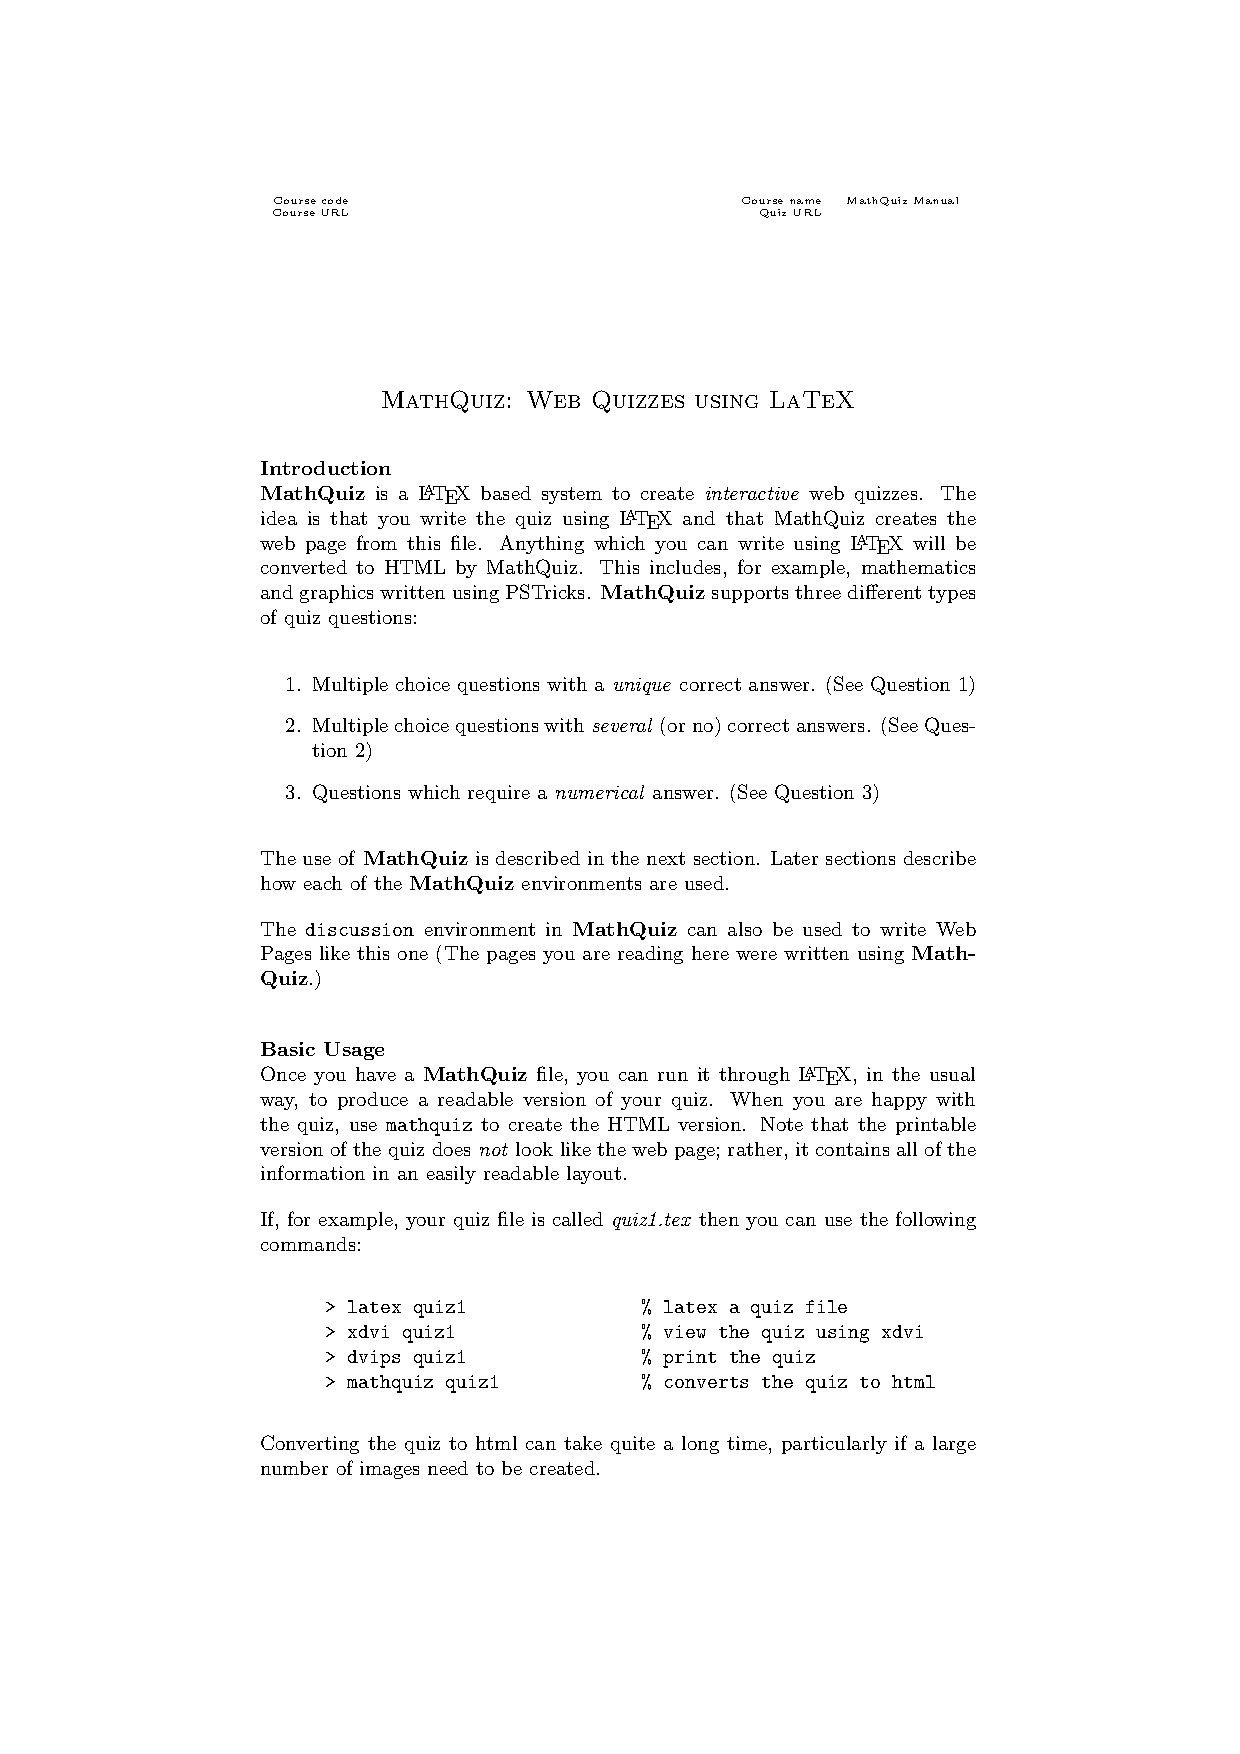
\includepdf[pages=-]{mathquiz-manual}

\begin{verbatim}
.. _`Andrew Mathas`: http://www.maths.usyd.edu.au/u/mathas/
.. _GPL: https://www.gnu.org/licenses/gpl-3.0.en.html
.. _LaTeX: https://www.latex-project.org/
.. _MathQuiz: http://www.maths.usyd.edu.au/u/MOW/MathQuiz/doc/mathquiz-manual.html
.. _Python: https://www.python.org
.. _TeX4ht: http://www.tug.org/tex4ht/
.. _texlive: https://www.tug.org/texlive/
\end{verbatim}

\section{Licence}

Copyright (C) 2013-2017

GNU General Public License, Version 3, 29 June 2007

This program is free software: you can redistribute it and/or modify it under
the terms of the GNU General Public License (GPL) as published by the Free
Software Foundation, either version 3 of the License, or (at your option) any
later version.

This program is distributed in the hope that it will be useful, but WITHOUT ANY
WARRANTY; without even the implied warranty of MERCHANTABILITY or FITNESS FOR A
PARTICULAR PURPOSE.  See the GNU General Public License for more details.

\end{document}
